\documentclass[10pt]{beamer}

\usepackage[utf8]{inputenc}
\usepackage{algorithm,algorithmic}
\usepackage{changepage}
\usepackage{amsmath}
\usepackage{comment}
\usepackage{graphicx}
\usepackage{media9}

\setbeamersize{text margin left=5mm,text margin right=5mm} 

\AtBeginSection[]{
  \begin{frame}
  \vfill
  \centering
  \begin{beamercolorbox}[sep=8pt,center,shadow=true,rounded=true]{title}
    \usebeamerfont{title}\insertsectionhead\par%
  \end{beamercolorbox}
  \vfill
  \end{frame}
}

\title[Inverse Reinforcement Learning Tool for Minigrid environment] %optional
{Inverse Reinforcement Learning Tool \\ for Minigrid environment }

\author[Giulio Bazzanti, Niccolò Biondi] % (optional, for multiple authors)
{Giulio~Bazzanti \and Niccolò~Biondi}

\date[HCI 2020] % (optional)
{Human Computer Interaction, 2020, March 5}

\usetheme[subsection=False]{Ilmenau}
\usecolortheme{beaver}
\setbeamercovered{invisible}

\begin{document}
\frame{\titlepage}

\begin{frame}
\frametitle{Table of Contents}
\tableofcontents
\end{frame}

\section{Introdution}
Reinforcement Learning (RL) is an area of machine learning concerned with how a particular artificial agent makes several actions inside an environment in order to maximize some cumulative rewards. With this kind of technique, the agent has the possibility to learn the right behavior to adopt in a certain environment through the \textsl{trial-and-error} mechanism. To achieve these goals, a policy network (the agent behavior) is defined and it takes the current environment state to perform the best action in the environment. Nowadays, the RL achieves superhuman performance in a range of environments, but requires that a designer manually specify a reward function.

In the Inverse Reinforcement Learning (IRL), the policy does not receive the reward directly from the environment during the training process. Instead,  we assume that there is a human in the loop who has an intention for the agent’s task, and communicates this intention to the agent using one the preferences feedback channel.  If the policy model mimics the human expert’s behavior well, it can achieve the performance of the human on the task. In this project, we implement the Inverse Reinforcement Learning method described in\ \cite{NIPS2018_8025} to train a policy agent to achieve the goal in the \textsl{Minigrid} environment\ \cite{gym_minigrid}. We use this kind of simple environment because, unlike is described in the original algorithm, we don't use a set of human demonstrations provided by an expert to pretrain the policy. In our case we use only the preferences, the human labels\ \cite{NIPS2018_8025}, provided by the user to define a reward model function which will give rewards for policy training. This choice allows us to train simultaneously the policy and the reward model. 
The human labels are collected thanks to a simple application, where the user can specify his preference between pairs of small segments of agent trajectories.
 
 In video games, the RL is used to define the Non-Player Characters (NPCs), that sometimes have superhuman abilities, overcoming the player skills. On the other hand, the RL can produce a predictable NPCs, making the game experience boring. So, in these cases, the players will not be involved in the game, abandoning it. 
 
 The scope of our project is to propose an IRL tool with which the video game designers can control the NPCs (agents) behaviour in order to create more interactive and engaging video games.
 

\section{Proposed Method}

\begin{frame}{Proposed method}

\begin{algorithm}[H]
\caption{Training Protocol \footnote{\href{http://papers.nips.cc/paper/8025-reward-learning-from-human-preferences-and-demonstrations-in-atari}{\color{blue}{Reward learning from human preferences and demonstrations in Atari, \textit{Ibarz et all.}}}}}

\begin{algorithmic}[1]
\STATE Run the policy in the environment and store "initial trajectories".
\STATE The annotator annotated all the "initial clips" and create the annotation buffer.
\STATE Pretrain the reward model from the annotation buffer.
\FOR{\textit{M} epochs} 
\STATE Train the policy in the environment for \textit{N} episodes with rewards from the reward model.
\STATE Sample pairs of clips from the resulting trajectories.
\STATE The annotator labels the selected pairs and puts them in the annotation buffer.
\STATE Train the reward model for \textit{K} batches from the annotation buffer.
\ENDFOR 
\end{algorithmic}
\end{algorithm}

\end{frame}

\begin{frame}
\frametitle{Policy}

\begin{itemize}
    %\item The policy receive an observation \textit{$o_t$} and it takes an action \textit{$a_t$}
    \item The reward is not taken from the environment but from a reward model
    \item The policy receives the current agent state as input and probabilities of actions as output
        
\end{itemize}

\centering
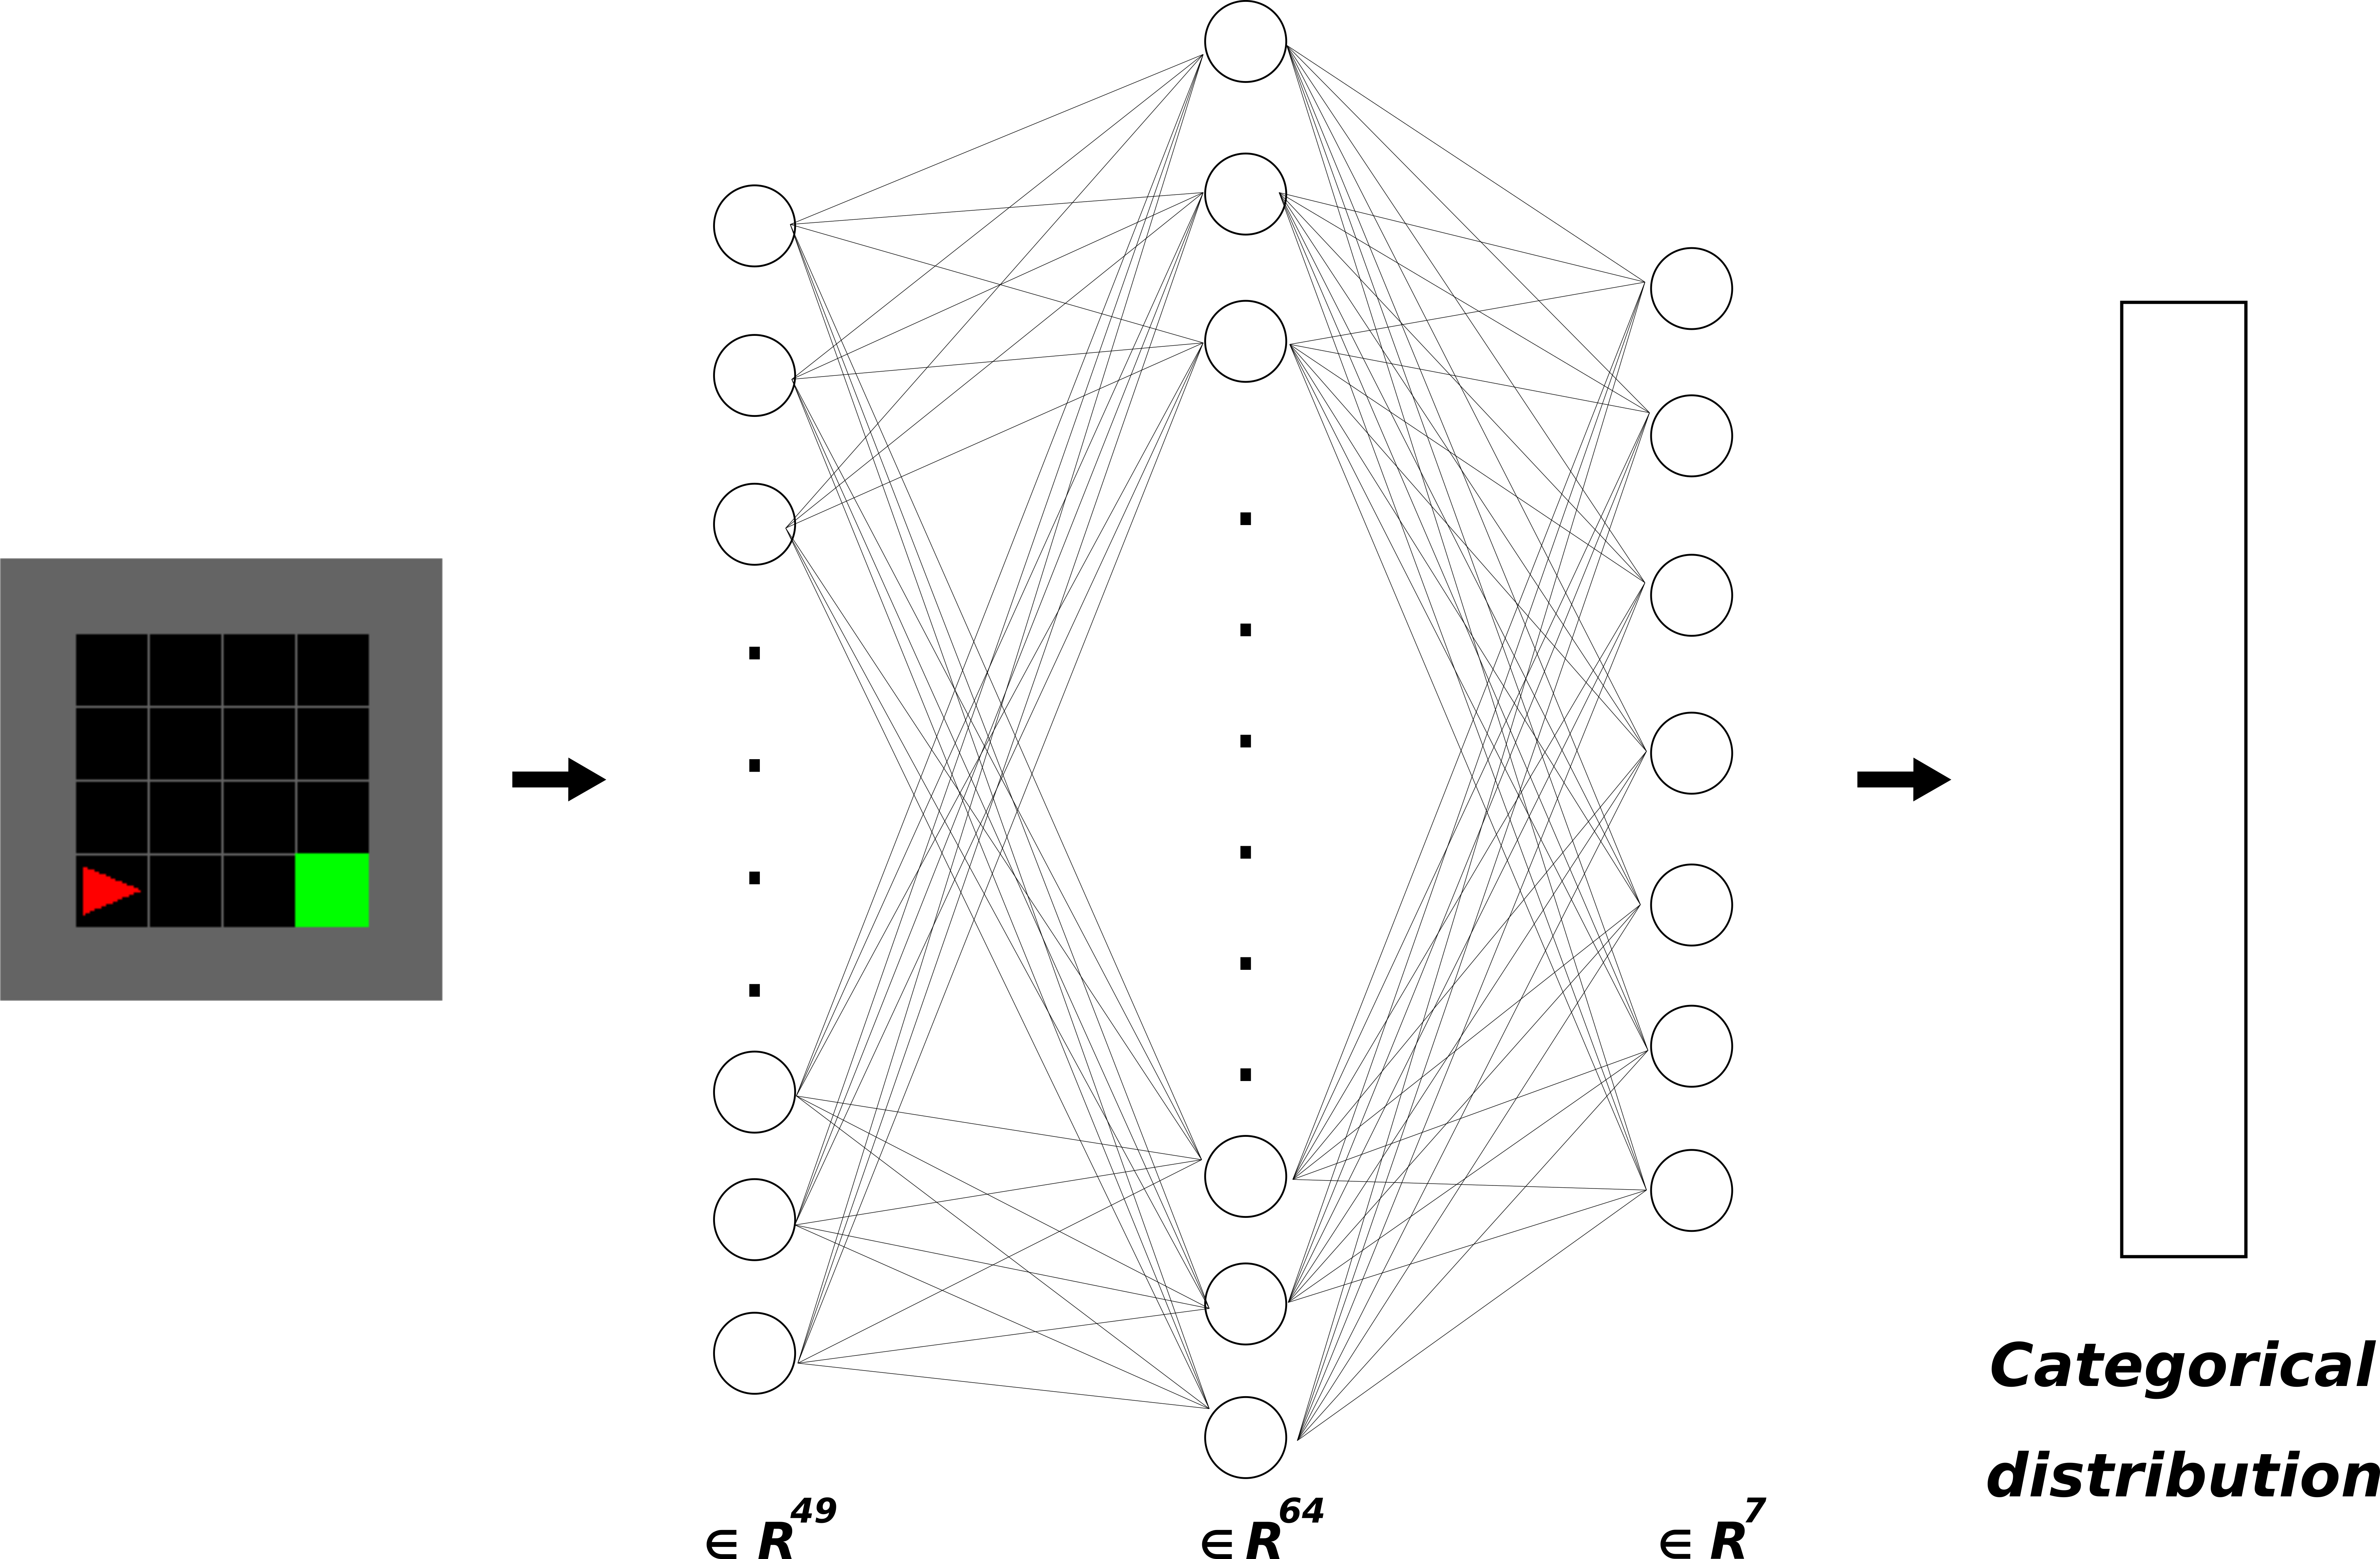
\includegraphics[width=0.6\linewidth]{images/policy.png}

\end{frame}

\begin{frame}
\frametitle{Annotator}
		\begin{itemize}
		\item The annotator gives preference feedback about pairs of clips
		\vspace{0.2cm}
		\begin{itemize}
			\item (0,1) (1,0) preferred clips
			\item (0.5,0.5) indifferent labels
			\item (0,0) discarded clips
		\end{itemize}
		
	\vspace{0.3cm}
	
		\item<2-> Human annotator vs Artificial annotator (\textit{Oracle})
		
	\end{itemize}
	\begin{columns}<2->
		\begin{column}{0.5\textwidth}
			\centering
			\footnotesize{
			\begin{tabular}{|c|c|c|c|}
				\hline
				1 & 0    & 0    & 0     \\ \hline
				1 & 0.5  & 0.25 & 0.125 \\ \hline
				1 & 0.25 & 0.5  & 0.125 \\ \hline
				1 & 1    & 1    & 10    \\ \hline
			\end{tabular}
		}
		\end{column}
		
		\begin{column}{0.5\textwidth}
			\centering
			\footnotesize{
			\begin{tabular}{|c|c|c|c|}
				\hline
				1 & 0 & 0 & 0  \\ \hline
				1 & 0 & 0 & 0  \\ \hline
				1 & 0 & 0 & 0  \\ \hline
				1 & 1 & 1 & 10 \\ \hline
			\end{tabular}
		}
		\end{column}
	\end{columns}
	
	\vspace{0.3cm}
	
	\begin{itemize}
		\item<3-> All the preferences are stored in the Annotation Buffer
	\end{itemize}
	
\end{frame}

\begin{frame}
\frametitle{Reward Model}
\begin{itemize}
    \item The Reward Model has to emulate the annotator labels
    \item It is trained to minimize the cross-entropy loss between predictions and labels
\end{itemize}

\vspace{0.2cm}

\begin{equation*}
    loss(\hat{r}) = - \sum_{(\sigma^1,\sigma^2,\mu)\in A} \mu(1)log(\hat{P}[\sigma^1 \succ \sigma^2]) + \mu(2)log(\hat{P}[\sigma^2 \succ \sigma^1])
\end{equation*}

%\vspace{0.3cm}
\begin{itemize}
    \item where
\end{itemize}

\begin{equation*}
    \hat{P}[\sigma^1 \succ \sigma^2] = \frac{exp(\sum_{o \in \sigma^1} \hat{r}(o))}{exp(\sum_{o \in \sigma^1} \hat{r}(o) + \sum_{o \in \sigma^2} \hat{r}(o))}
\end{equation*}



\end{frame}


\begin{frame}
\frametitle{Reward Model}
\begin{itemize}
    \item The Reward Model predicts a list of rewards from a clip
\end{itemize}
\vspace{0.3cm}
\centering
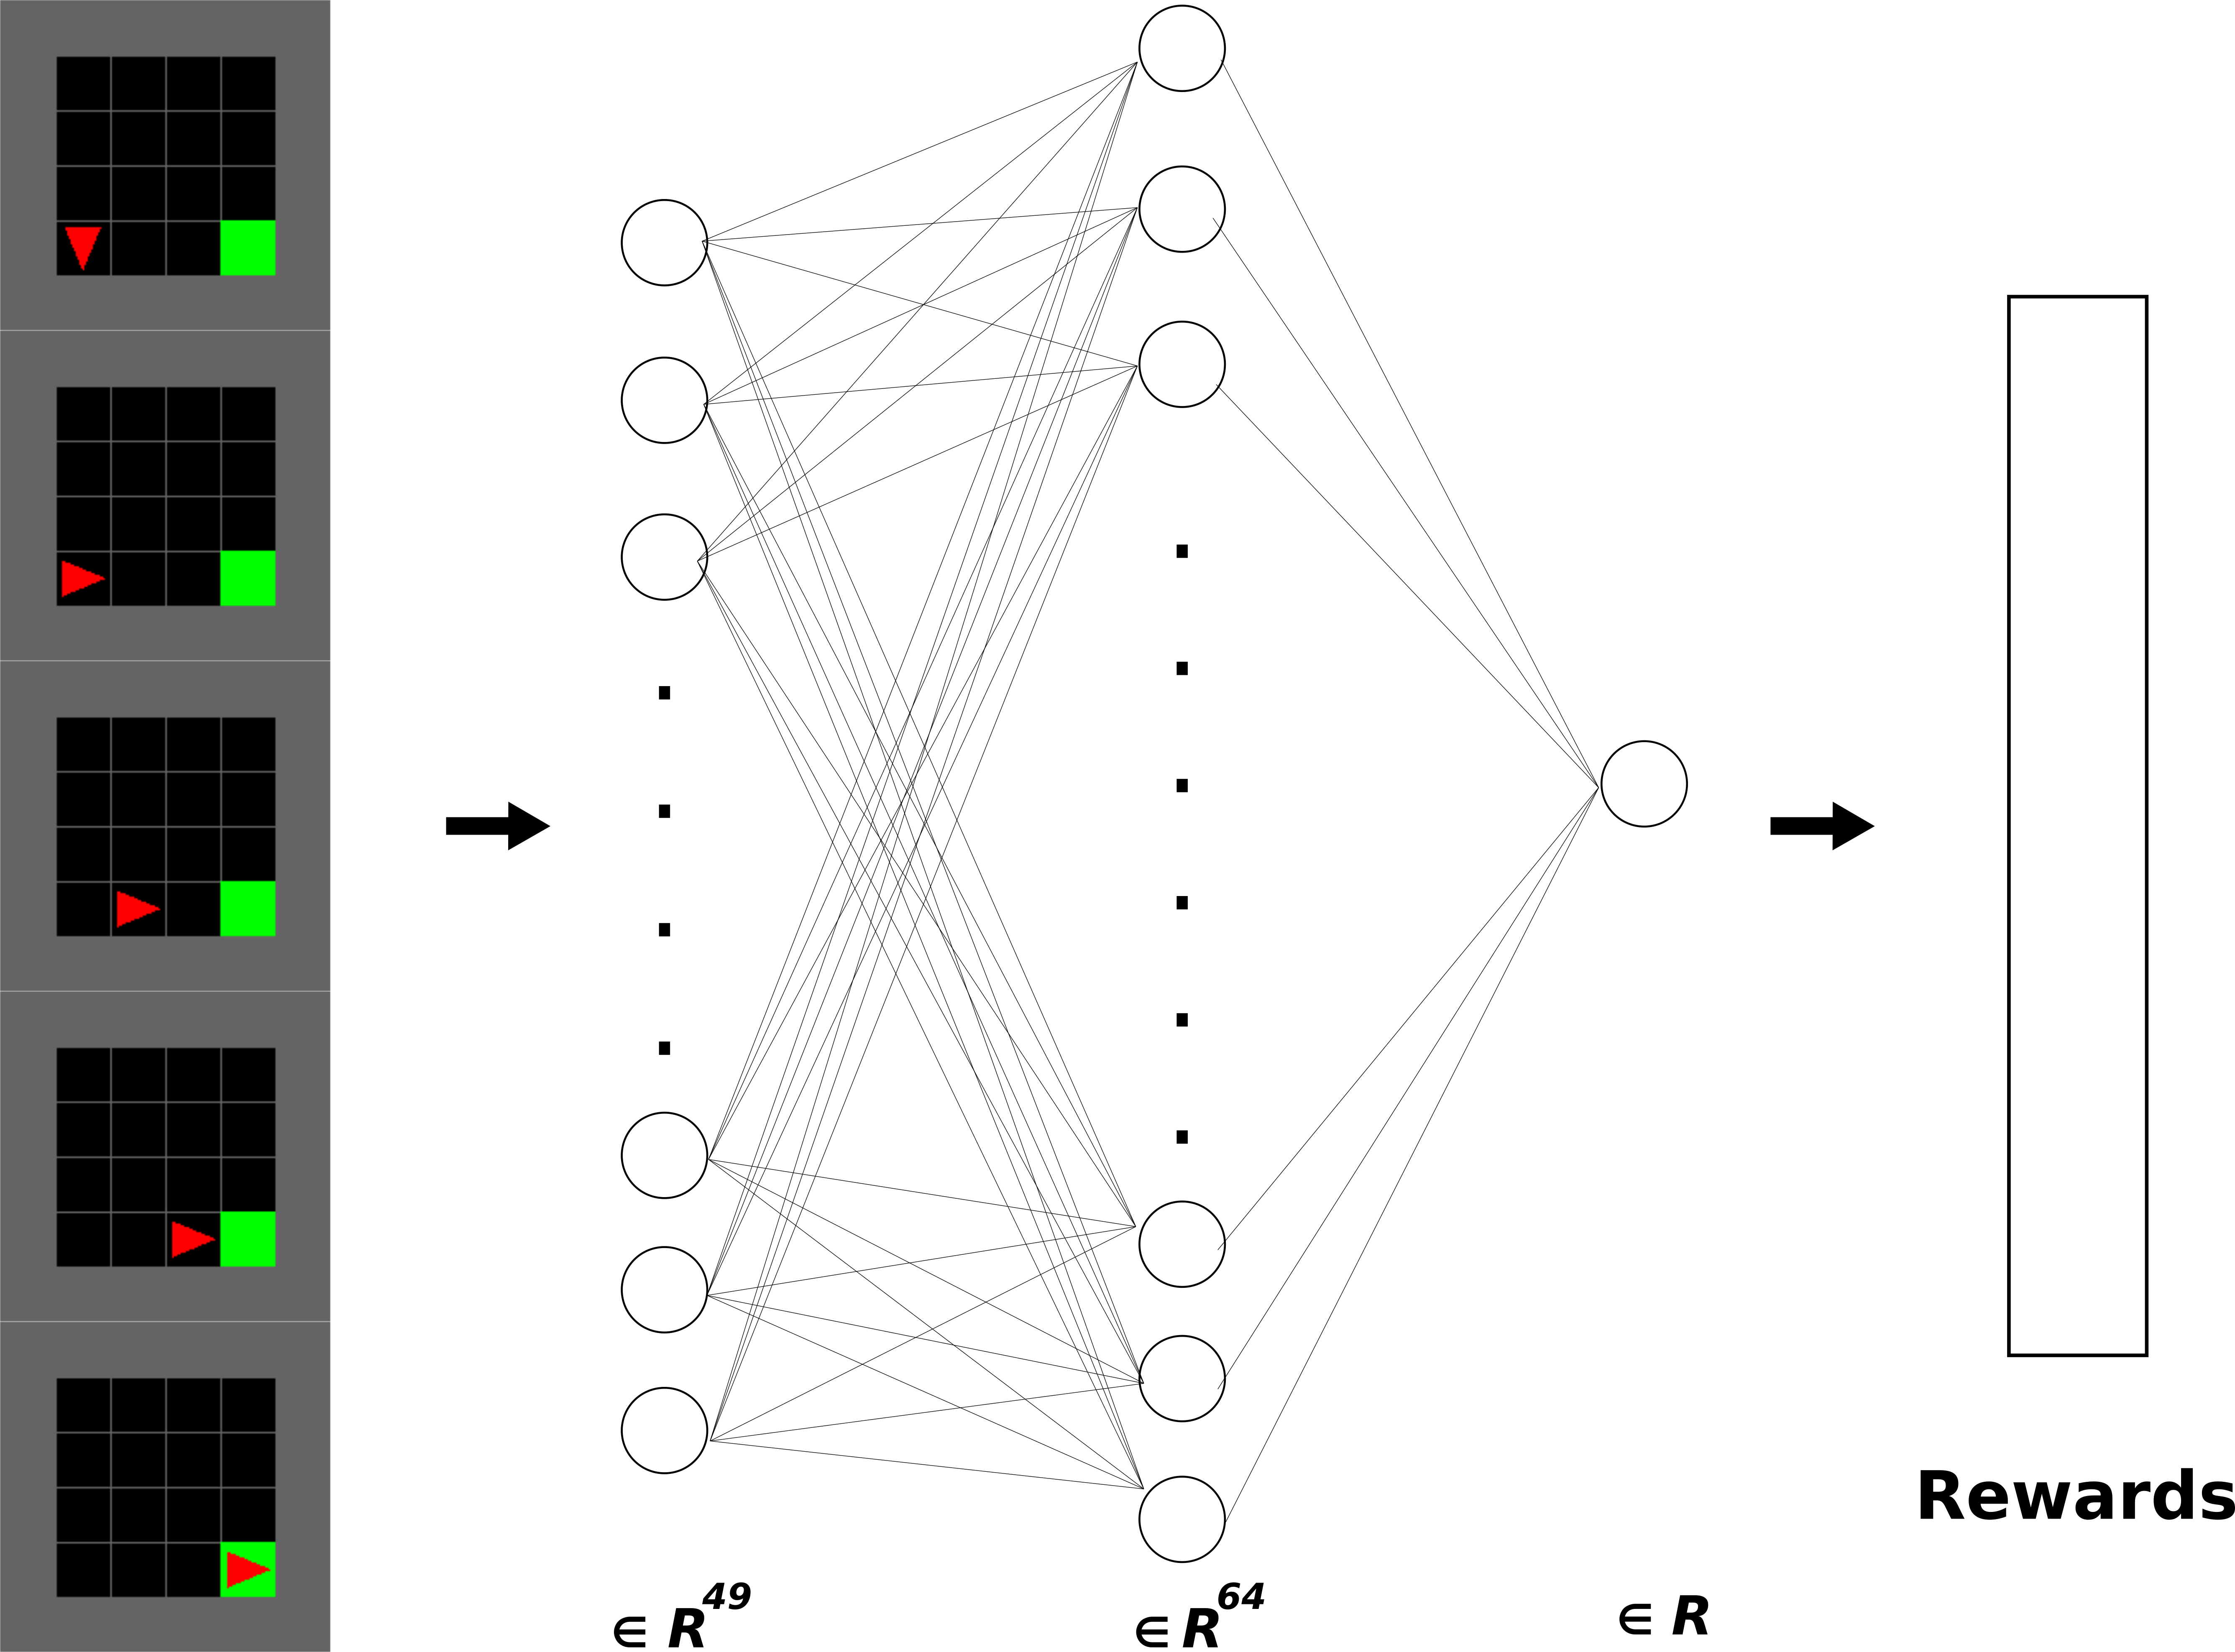
\includegraphics[width=0.55\linewidth]{images/reward.png}
\end{frame}


\begin{comment}
\subsection{IRL Components}

\begin{frame}
\frametitle{Policy}
dasdsa
\end{frame}

\begin{frame}
\frametitle{Annotator}
dasdsa
\end{frame}

\begin{frame}
\frametitle{Reward model}
\begin{itemize}
    \item bello
    \item raga
\end{itemize}
\end{frame}

\end{comment}



\section{IRL Tool}

\begin{frame}{Motivations}
	\begin{itemize}
		\item
		\item
	\end{itemize}
\end{frame}

\begin{frame}{Set Up Window}
	\centering
   \includemedia[width=0.75\linewidth, keepaspectratio, passcontext, noplaybutton,
   activate=pageopen,
   transparent, addresource=videos/tool.mp4,
   flashvars={source=videos/tool.mp4&autoPlay=true&loop=true}
   ]{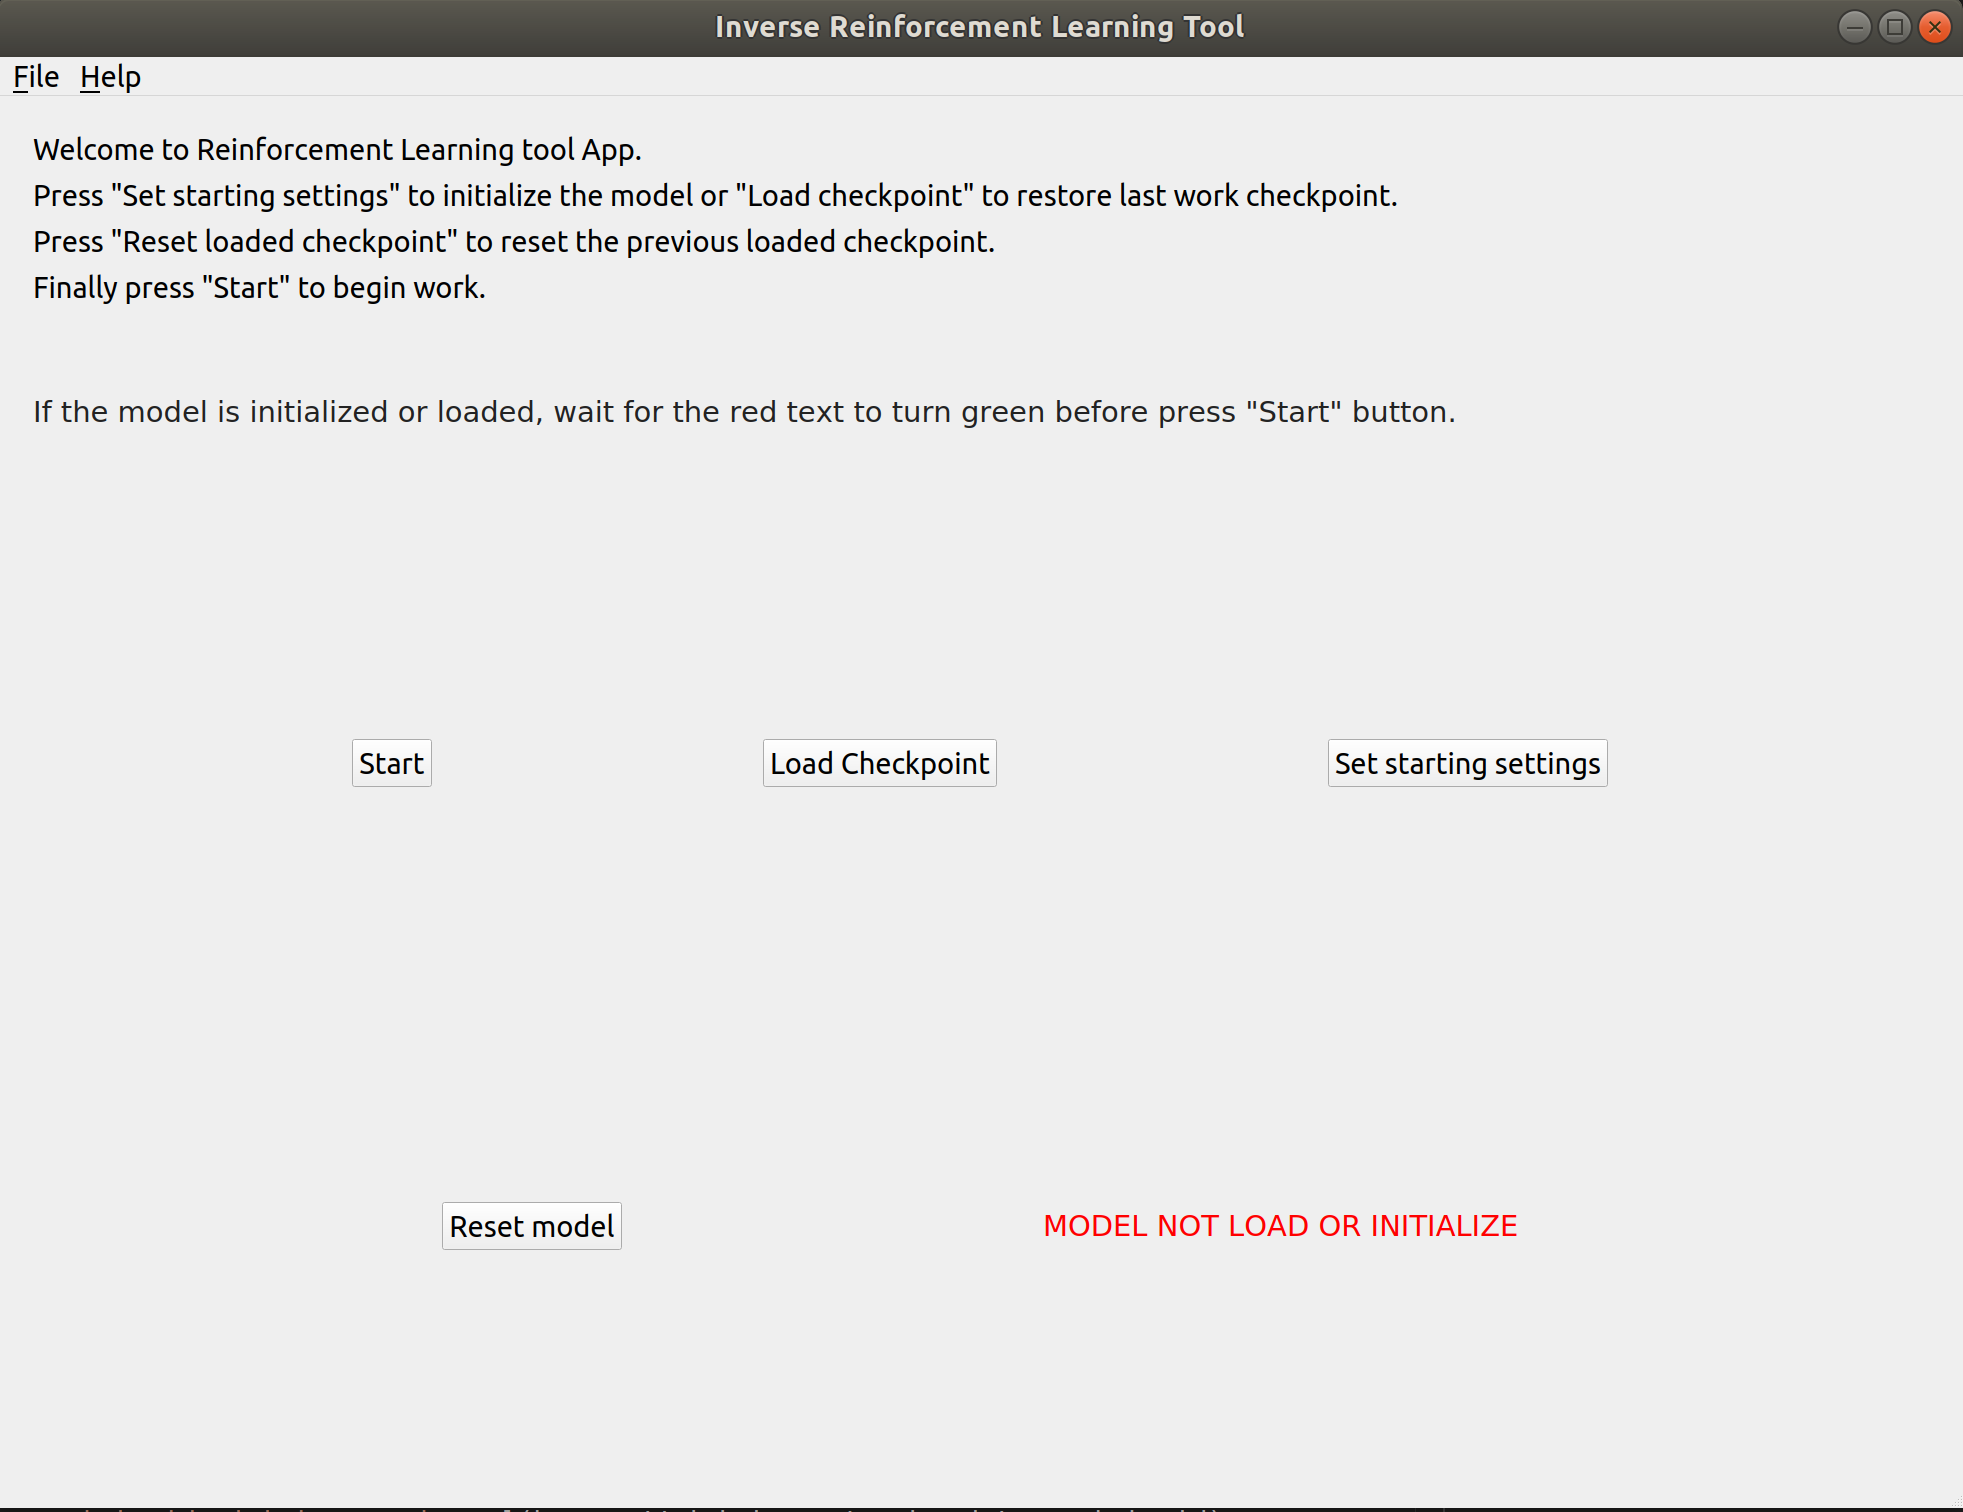
\includegraphics[width=0.75\linewidth]{videos/tool.png}}{VPlayer.swf}
\end{frame}

\begin{frame}{Training iteration}
	\centering
	\includemedia[width=0.75\linewidth, keepaspectratio, passcontext,
	activate=pageopen, noplaybutton,
	transparent, addresource=videos/alg.mp4,
	flashvars={source=videos/alg.mp4&autoPlay=true&loop=true}
	]{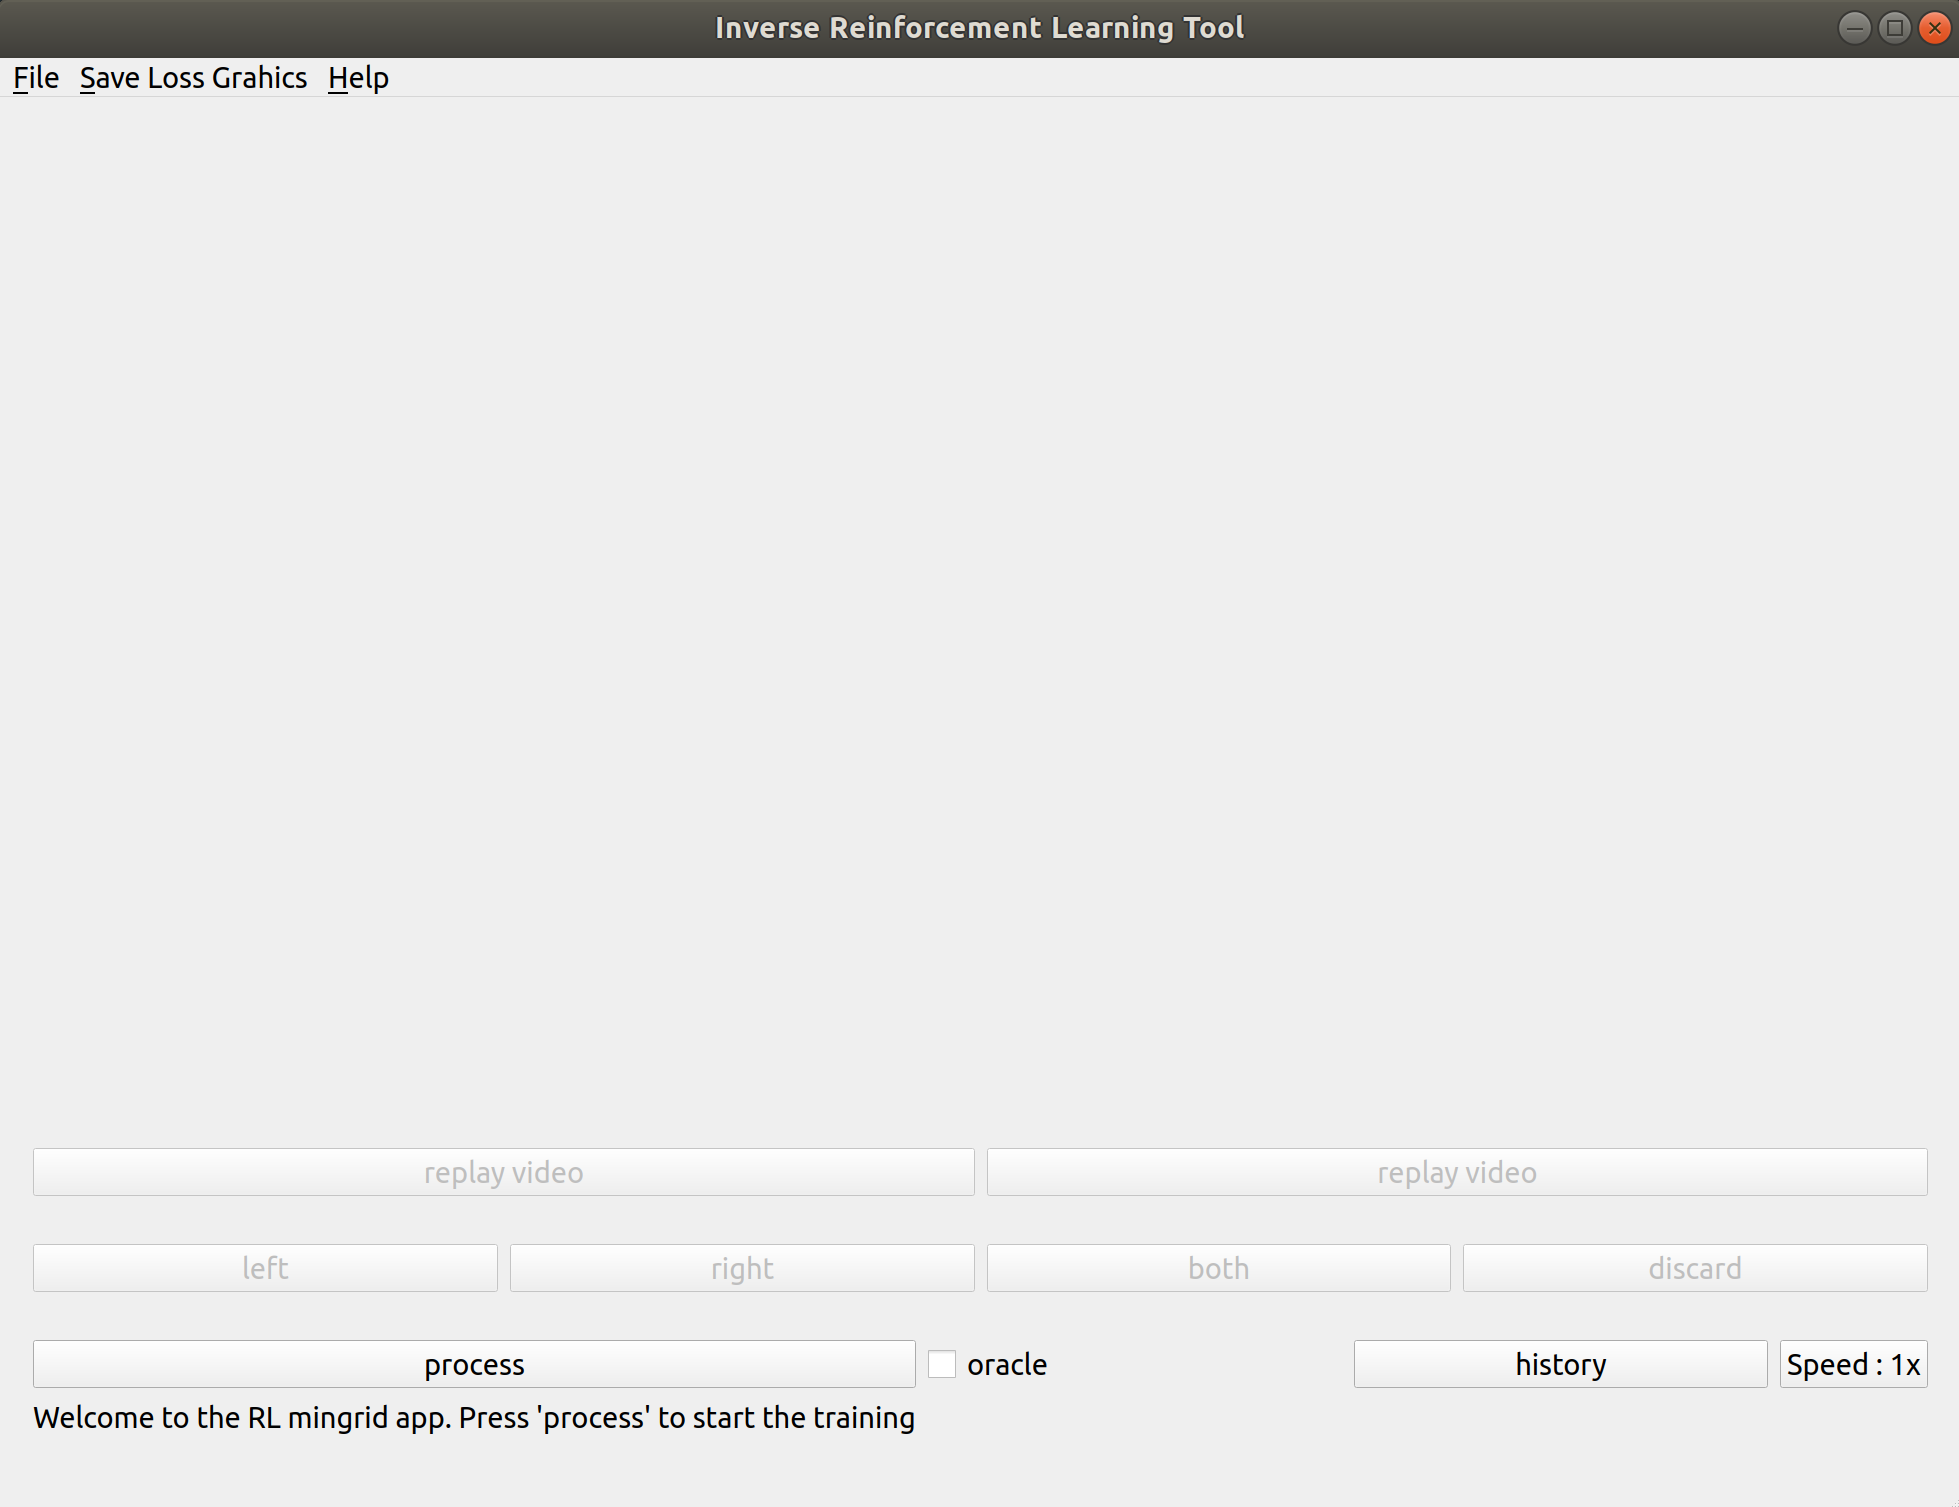
\includegraphics[width=0.75\linewidth]{videos/alg.png}}{VPlayer.swf}
\end{frame}
\section{Experimental Results}

% Minigrid slide
\begin{frame}{MiniGrid Environment}

\begin{columns}
        \begin{column}{0.6\textwidth}
        \small{        
            \begin{itemize}
                \item 6x6 Empty MiniGrid environment for experiments
                \item Optimal trajectory achieved with RL
            \end{itemize}
        }
            
        \end{column}
        \begin{column}{0.4\textwidth}
        \includemedia[width=0.7\linewidth, keepaspectratio, noplaybutton,
            passcontext,transparent,addresource=videos/RLmvs.mp4,
            flashvars={source=videos/RLmvs.mp4&autoPlay=true&loop=true}
            ]{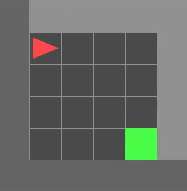
\includegraphics[width=0.7\linewidth]{videos/RLmvs-1.png}}{VPlayer.swf}
        \end{column}
        
    \end{columns}

\begin{columns}<2->
        \begin{column}{0.6\textwidth}
        \small{        
            \begin{itemize}
                \item Sub-optimal trajectory forced with IRL
                \item The user controls the agent behaviour
            \end{itemize}
        }
            
        \end{column}
        \begin{column}{0.4\textwidth}
            \includemedia[width=0.7\linewidth, keepaspectratio, passcontext,
                transparent, addresource=videos/IRLmvs.mp4, noplaybutton,
                flashvars={source=videos/IRLmvs.mp4&autoPlay=true&loop=true}
                ]{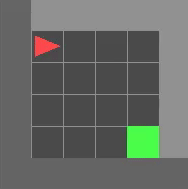
\includegraphics[width=0.7\linewidth]{videos/IRLmvs-1.png}}{VPlayer.swf}
        \end{column}
        
    \end{columns}
    
\end{frame}

% Tuning slide
\begin{frame}{Tuning the components}
    \begin{itemize}
        \item Policy
        \begin{itemize}
            \item the agent has to reach easily the  environment goal $\Rightarrow$ episode length 150
            \item no negative goal reward or big values range $\Rightarrow$ standard deviation 0.5 
        \end{itemize} 

        \vspace{0.2cm}
        \pause
        \item Annotator
        \begin{itemize}
            \item sparse vs dense Oracle
        \end{itemize}
        
        \vspace{0.2cm}
        \pause
        \item Reward Model
        \begin{itemize}
            \item variable K batch vs constant K batch
            \item early stopping and decreasing annotations
        \end{itemize}
    \end{itemize}
\end{frame}

% Reward model loss
\begin{frame}{Reward Model Loss}

    \begin{itemize}
        \item The reward model loss grows during the training protocol.
    \end{itemize}
    \centering
    \vspace{0.4cm}
    \includegraphics<1>[width=0.6\linewidth]{images/reward_loss.png}
    
    
\end{frame}

% Reward model loss
\begin{frame}{}
\centering

\includegraphics[width=1\linewidth]{images/bothlosses.png}

\begin{adjustwidth}{-2em}{-2em}
    \begin{columns}
        \begin{column}{0.5\textwidth}
        \small{        
            \begin{itemize}
                \item Small contribution to total loss
                \item Same range during all the training
            \end{itemize}
        }
            
        \end{column}
        \begin{column}{0.5\textwidth}
        \small{
            \begin{itemize}
                \item Big contribution to total loss
                \item The number of those preferences make the loss grow
            \end{itemize}
        }
        
        \end{column}
        
    \end{columns}
\end{adjustwidth}

\begin{equation*}
loss(\hat{r}) = - \sum_{(\sigma^1,\sigma^2,\mu)\in A} \mu(1)log(\hat{P}[\sigma^1 \succ \sigma^2]) + \mu(2)log(\hat{P}[\sigma^2 \succ \sigma^1])
\end{equation*}

\end{frame}


\section{Conclusions}

\begin{frame}{Conclusions and Future Works}

\begin{itemize}
	\item For now \ldots
	\begin{itemize}
		\item A not-expert user can build an IRL system
		\item The agent learns sub-optimal trajectory 
		\item Better NPCs creation
	\end{itemize}
	\vspace{0.5cm}
	\item \ldots then
	\begin{itemize}
		\item More complex environment to increase IRL benefits
		\item Process environment images with agent states (with CNN and/or LSTM)
	\end{itemize}
\end{itemize}

\end{frame}


%\setbeamertemplate{footbar}{\insertframenumber}


\end{document}